\subsubsection{Primer 4 - Iks Oks}

\large{1. Opis zadatka}
\normalsize

Napraviti Client-Server aplikaciju koja će komunicirati na TCP portu X (gde je $X = broj\ indeksa/24 + 2000$) i omogućavati klijentima da igraju igru iks-oks.

\large{2. Opis igre}
\normalsize

Iks-oks je igra za dva igrača koja koristi kockice i tablu sa $3\times3$ polja. Igrači neizmenično postavljaju znakove X (Igrač koji ima prvi potez) ili O na tablu sve dok ne postave znakove na tri uzastopna mesta po redovima, kolonama ili dijagonalama. Ukoliko su sva polja popunjena a ni jedan igrač nije ostvario uslov za pobedu, igra je nerešena. Nakon kraja igre može se desiti revanš ukoliko oba igrača žele.

\large{3. Specifikacija zadatka}
\normalsize

Aplikacija treba da podrži konekciju \textbf{maksimalno} 2 klijenta. Nakon početka aplikacije klijent 1 će predstavljati igrača 1 (Igrač 1 ima prvi potez). Igra počinje kada oba klijenta pošalju poruku "start". Nakon poslate poruke, klijent čeka povratnu poruku od servera koja potvrđuje početak igre. Nakon početka igre, server obaveštava klijenta koji je njegov simbol, X ako je igrač 1 a O ako je igrač 2. Na početku svake runde server klijentu šalje trenutno stanje table. Klijent bira polje na kom polju želi da postavi znak u formatu $[i,j]$. Server proverava validnost poteza (Nije moguće postavljanje simbola na već popunjeno polje) i validnost poruke. Ukoliko je došlo do greške, server je ispisuje i traži od korisnika da unese opet željeno polje. Po završetku runde server obaveštava klijente ko je pobednik ili da je igra ne rešena, nakon čega im nudi revanš. Klijenti mogu da pošalju D ukoliko žele revanš ili N ako ne žele. Oba klijenta moraju da se slože za revanš nakon čega im se prezentuje prazna tabla i igraju ispočetka, u suprotnom se igra prekida.

\begin{figure}[H]
    \centering
    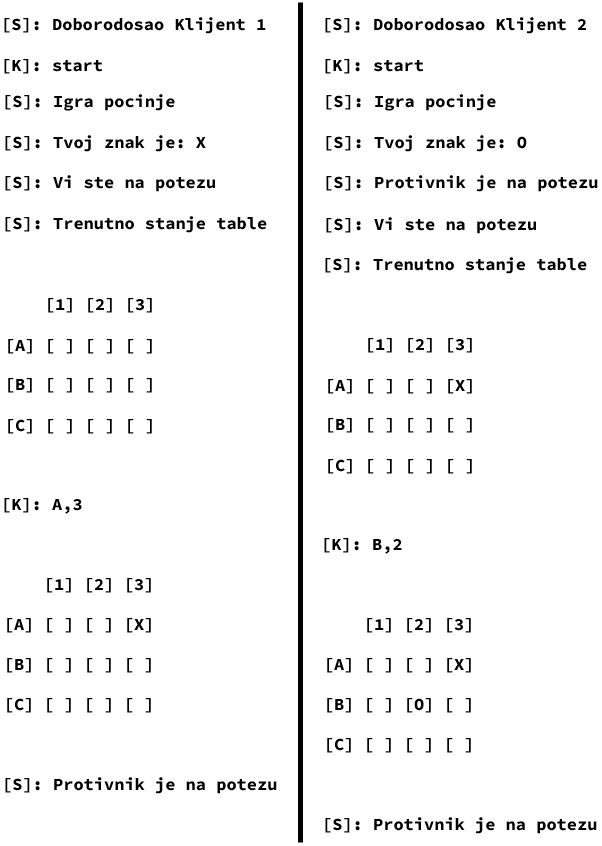
\includegraphics[width=0.5\textwidth]{Slike/XO/XO_Pocetak.png}
    \caption*{Primer pocetka igre. (Levo) Interakcija od strane Klijenta 1. (Desno) Interakcija od strane Klijenta 2}
    \label{fig:xo_pocetak}
\end{figure}